\documentclass[aspectratio=169,12pt,t]{beamer}

% --- Theme: Metropolis (modern, clean) ---
\usetheme[progressbar=frametitle,numbering=fraction,block=fill]{metropolis}

% --- Fira Sans font (install texlive-fonts-extra if missing) ---
\IfFileExists{FiraSans.sty}{\usepackage[sfdefault]{FiraSans}}{}

% --- Light background with warm accent ---
\definecolor{mDarkTeal}{RGB}{35,55,59}
\definecolor{mLightBrown}{RGB}{235,228,216}
\definecolor{mAccent}{RGB}{140,70,20}

\setbeamercolor{normal text}{fg=mDarkTeal,bg=white}
\setbeamercolor{alerted text}{fg=mAccent}
\setbeamercolor{frametitle}{bg=mDarkTeal,fg=white}
\setbeamercolor{progress bar}{fg=mAccent,bg=mLightBrown}
\setbeamercolor{title separator}{fg=mAccent}
\setbeamercolor{progress bar in head/foot}{fg=mAccent,bg=mLightBrown}
\setbeamercolor{progress bar in section page}{fg=mAccent,bg=mLightBrown}

% --- Packages ---
\usepackage[utf8]{inputenc}
\usepackage{amsmath,amssymb,amsthm}
\usepackage{mathrsfs}
\usepackage{tikz}
\usetikzlibrary{arrows.meta,positioning,calc,decorations.pathreplacing,shapes,patterns}
\usepackage{pgfplots}
\pgfplotsset{compat=1.18}

% --- Custom colors for content types ---
\definecolor{defcolor}{RGB}{25,85,120}
\definecolor{thmcolor}{RGB}{140,35,35}
\definecolor{proofcolor}{RGB}{35,100,50}
\definecolor{excolor}{RGB}{140,75,10}
\definecolor{remcolor}{RGB}{90,90,90}

% --- Beamer blocks for mathematical content types ---
\newenvironment{defblock}[1]{%
  \setbeamercolor{block title}{bg=defcolor,fg=white}%
  \setbeamercolor{block body}{bg=defcolor!5}%
  \begin{block}{#1}}{\end{block}}

\newenvironment{thmblock}[1]{%
  \setbeamercolor{block title}{bg=thmcolor,fg=white}%
  \setbeamercolor{block body}{bg=thmcolor!5}%
  \begin{block}{#1}}{\end{block}}

\newenvironment{proofblock}[1]{%
  \setbeamercolor{block title}{bg=proofcolor,fg=white}%
  \setbeamercolor{block body}{bg=proofcolor!5}%
  \begin{block}{#1}}{\end{block}}

\newenvironment{exblock}[1]{%
  \setbeamercolor{block title}{bg=excolor,fg=white}%
  \setbeamercolor{block body}{bg=excolor!5}%
  \begin{block}{#1}}{\end{block}}

\newenvironment{remblock}[1]{%
  \setbeamercolor{block title}{bg=remcolor,fg=white}%
  \setbeamercolor{block body}{bg=remcolor!5}%
  \begin{block}{#1}}{\end{block}}

% --- Metadata ---
\title{Chapter 1: The Real and Complex Number Systems}
\subtitle{Section: Appendix --- Construction of the Real Numbers}
\author{Based on Walter Rudin's \emph{Principles of Mathematical Analysis}}
\date{}

\begin{document}

% =============================================================================
% TITLE AND OUTLINE
% =============================================================================

\begin{frame}
  \titlepage
  \note{
    Welcome to Chapter 1, Section 8: the Appendix. This is one of the most
    important sections in the entire book, where we actually construct the real
    numbers from the rationals. In Theorem 1.19, Rudin stated that there exists
    an ordered field with the least-upper-bound property. Now we prove it, step
    by step, using the elegant method of Dedekind cuts.
  }
\end{frame}

\begin{frame}{Outline}
  \tableofcontents
  \note{
    Here is the roadmap for this appendix. We will go through the construction
    in nine steps, starting with the definition of Dedekind cuts, then building
    up the order structure, the least-upper-bound property, addition,
    multiplication, and finally the embedding of the rationals into the reals.
    Let's get started.
  }
\end{frame}

% =============================================================================
% MOTIVATION
% =============================================================================

\section{Motivation and Overview}

% --- Recall Theorem 1.19 ---
\begin{frame}{Recall: Theorem 1.19}
  \begin{alertblock}{Theorem 1.19}
    There exists an ordered field $\mathbb{R}$ which has the least-upper-bound
    property. Moreover, $\mathbb{Q}$ is a subfield of $\mathbb{R}$.
  \end{alertblock}

  \vspace{0.5em}
  This was \emph{stated} earlier without proof. The entire appendix is devoted
  to \alert{proving} this theorem.

  \note{
    Before we dive in, let's recall exactly what we are trying to prove.
    Theorem 1.19 makes two claims: first, that there exists an ordered field
    with the least-upper-bound property; and second, that the rationals sit
    inside it as a subfield. We accepted this on faith earlier, but now we
    will construct such a field explicitly.
  }
\end{frame}

% --- Build 1/3 ---
\begin{frame}{Why This Appendix Matters}
  \begin{itemize}
    \item Theorem 1.19 \emph{asserts} that an ordered field with the
          least-upper-bound property exists
  \end{itemize}

  \note{
    So far in this chapter, we have been working with the real numbers as if
    they exist. Theorem 1.19 claimed that there is an ordered field with the
    least-upper-bound property, but we never proved it. This appendix fills
    that gap. Let's outline the strategy.
  }
\end{frame}

% --- Build 2/3 ---
\begin{frame}{Why This Appendix Matters}
  \begin{itemize}
    \item Theorem 1.19 \emph{asserts} that an ordered field with the
          least-upper-bound property exists
    \item This appendix provides the \alert{explicit construction} of $\mathbb{R}$
          from $\mathbb{Q}$
  \end{itemize}

  \note{
    We are going to actually build the real numbers out of the rationals. This
    is not just an abstract existence argument. We will define specific objects,
    called Dedekind cuts, and equip them with addition, multiplication, and
    order. And the method has a name.
  }
\end{frame}

% --- Build 3/3 ---
\begin{frame}{Why This Appendix Matters}
  \begin{itemize}
    \item Theorem 1.19 \emph{asserts} that an ordered field with the
          least-upper-bound property exists
    \item This appendix provides the \alert{explicit construction} of $\mathbb{R}$
          from $\mathbb{Q}$
    \item The method: \alert{Dedekind cuts} --- invented by Richard Dedekind in 1872
  \end{itemize}

  \note{
    The tool we use is called a Dedekind cut, named after the German
    mathematician Richard Dedekind, who published this construction in 1872.
    Around the same time, Georg Cantor independently gave a different
    construction using Cauchy sequences. Both approaches achieve the same goal:
    filling in the gaps of the rational number line. Let's see how cuts work.
  }
\end{frame}

% --- Construction roadmap Build 1/4 ---
\begin{frame}{Construction Roadmap}
  \begin{description}[Steps 4--7:]
    \item[Steps 1--2:] Define cuts and order them $\;\longrightarrow\;$
          $\mathbb{R}$ is an \alert{ordered set}
  \end{description}

  \note{
    The construction proceeds in nine steps. In the first two steps, we define
    what a cut is and how to compare two cuts. This gives us an ordered set.
    Next comes the key property.
  }
\end{frame}

% --- Construction roadmap Build 2/4 ---
\begin{frame}{Construction Roadmap}
  \begin{description}[Steps 4--7:]
    \item[Steps 1--2:] Define cuts and order them $\;\longrightarrow\;$
          $\mathbb{R}$ is an \alert{ordered set}
    \item[Step 3:] Prove the \alert{least-upper-bound property}
  \end{description}

  \note{
    Step 3 is the heart of the construction. We show that the ordered set of
    cuts has the least-upper-bound property. This is the whole reason we use
    cuts --- they are designed to fill the gaps in the rationals. But an ordered
    set is not yet a field.
  }
\end{frame}

% --- Construction roadmap Build 3/4 ---
\begin{frame}{Construction Roadmap}
  \begin{description}[Steps 4--7:]
    \item[Steps 1--2:] Define cuts and order them $\;\longrightarrow\;$
          $\mathbb{R}$ is an \alert{ordered set}
    \item[Step 3:] Prove the \alert{least-upper-bound property}
    \item[Steps 4--7:] Define $+$ and $\cdot$ $\;\longrightarrow\;$
          $\mathbb{R}$ is an \alert{ordered field}
  \end{description}

  \note{
    Steps 4 through 7 equip the set of cuts with addition and multiplication,
    turning it into an ordered field. Addition is defined in detail;
    multiplication requires a bit more care because of signs. And finally, we
    need to connect the rationals to this new field.
  }
\end{frame}

% --- Construction roadmap Build 4/4 ---
\begin{frame}{Construction Roadmap}
  \begin{description}[Steps 4--7:]
    \item[Steps 1--2:] Define cuts and order them $\;\longrightarrow\;$
          $\mathbb{R}$ is an \alert{ordered set}
    \item[Step 3:] Prove the \alert{least-upper-bound property}
    \item[Steps 4--7:] Define $+$ and $\cdot$ $\;\longrightarrow\;$
          $\mathbb{R}$ is an \alert{ordered field}
    \item[Steps 8--9:] Embed $\mathbb{Q}$ into $\mathbb{R}$
          $\;\longrightarrow\;$ $\mathbb{Q}$ is a \alert{subfield} of $\mathbb{R}$
  \end{description}

  \note{
    Finally, Steps 8 and 9 show that the rationals sit naturally inside the
    reals. Each rational number "r" corresponds to a specific cut, and this
    correspondence preserves sums, products, and order. This is why we can
    regard the rationals as a subfield of the reals. Let's begin with Step 1.
  }
\end{frame}

% =============================================================================
% STEP 1: DEDEKIND CUTS
% =============================================================================

\section{Step 1: Dedekind Cuts}

\begin{frame}{The Big Idea: Cuts as Real Numbers}
  \begin{center}
  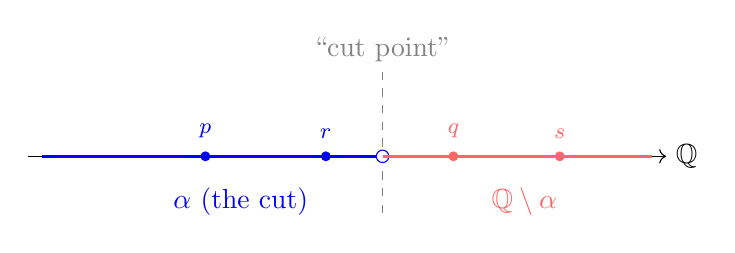
\begin{tikzpicture}[scale=0.9]
    % Number line
    \draw[->] (-1,0) -- (8,0) node[right]{$\mathbb{Q}$};

    % The cut point
    \draw[dashed, gray] (4,-.8) -- (4,1.2);
    \node[gray, above] at (4,1.2) {``cut point''};

    % Left part (the cut alpha)
    \draw[very thick, blue] (-0.8,0) -- (4,0);
    \draw[blue, fill=white] (4,0) circle (2.5pt);
    \node[blue, below=8pt] at (2,0) {$\alpha$ (the cut)};

    % Right part
    \draw[very thick, red!60] (4,0) -- (7.8,0);
    \node[red!60, below=8pt] at (6,0) {$\mathbb{Q} \setminus \alpha$};

    % Points
    \fill[blue] (1.5,0) circle (2pt) node[above=3pt]{\footnotesize$p$};
    \fill[blue] (3.2,0) circle (2pt) node[above=3pt]{\footnotesize$r$};
    \fill[red!60] (5,0) circle (2pt) node[above=3pt]{\footnotesize$q$};
    \fill[red!60] (6.5,0) circle (2pt) node[above=3pt]{\footnotesize$s$};
  \end{tikzpicture}
  \end{center}

  \vspace{0.3em}
  A \alert{cut} $\alpha$ is a subset of $\mathbb{Q}$ that is ``everything to
  the left'' of some dividing point.

  \note{
    Here is the central idea. Think of the rational number line. A Dedekind cut
    is a way of slicing this line into two pieces: a left piece and a right
    piece. The left piece, which we call "alpha", is the cut itself. Every
    rational "p" in the cut is less than every rational "q" not in the cut. The
    beautiful thing is that the dividing point does not have to be a rational
    number. This is exactly how cuts capture irrational numbers like the square
    root of 2. Let's make this precise.
  }
\end{frame}

% --- Definition of cut: Build 1/3 ---
\begin{frame}{Step 1: Definition of a Cut}
  \begin{defblock}{Definition: Cut (Dedekind Cut)}
    A \alert{cut} is a set $\alpha \subset \mathbb{Q}$ satisfying:
    \begin{enumerate}
      \item[\textbf{(I)}] $\alpha \neq \emptyset$ and $\alpha \neq \mathbb{Q}$
    \end{enumerate}
  \end{defblock}

  \note{
    Here is an honest question before we start: why would anyone think a
    subset of the rationals is a good way to represent a real number?
    The motivation is that a real number is determined by the rationals
    below it --- if you know exactly which rationals are less than "x", you
    know "x". So we cut out the middleman and simply declare the real
    number to be the set of rationals below it. The three axioms we
    are about to list just pin down what it means for a set to be "all
    rationals below some invisible point".
  }
\end{frame}

% --- Definition of cut: Build 2/3 ---
\begin{frame}{Step 1: Definition of a Cut}
  \begin{defblock}{Definition: Cut (Dedekind Cut)}
    A \alert{cut} is a set $\alpha \subset \mathbb{Q}$ satisfying:
    \begin{enumerate}
      \item[\textbf{(I)}] $\alpha \neq \emptyset$ and $\alpha \neq \mathbb{Q}$
      \item[\textbf{(II)}] If $p \in \alpha$, $q \in \mathbb{Q}$, and $q < p$,
            then $q \in \alpha$
    \end{enumerate}
  \end{defblock}

  \note{
    Property 2 rules out pathological subsets like "the even rationals" or
    "rationals with prime denominators". Such sets would have holes scattered
    everywhere and would not correspond to any point on the number line.
    Downward closure is what forces a cut to look like a solid ray stretching
    all the way to negative infinity, which is exactly the geometry we want.
  }
\end{frame}

% --- Definition of cut: Build 3/3 ---
\begin{frame}{Step 1: Definition of a Cut}
  \begin{defblock}{Definition: Cut (Dedekind Cut)}
    A \alert{cut} is a set $\alpha \subset \mathbb{Q}$ satisfying:
    \begin{enumerate}
      \item[\textbf{(I)}] $\alpha \neq \emptyset$ and $\alpha \neq \mathbb{Q}$
      \item[\textbf{(II)}] If $p \in \alpha$, $q \in \mathbb{Q}$, and $q < p$,
            then $q \in \alpha$
      \item[\textbf{(III)}] If $p \in \alpha$, then $p < r$ for some
            $r \in \alpha$
    \end{enumerate}
  \end{defblock}

  \vspace{0.3em}
  The members of $\mathbb{R}$ will be the cuts. Letters $p, q, r, \dots$ denote
  rationals; $\alpha, \beta, \gamma, \dots$ denote cuts.

  \note{
    Property 3 is subtle but essential. It is a technical convention that
    prevents every real number from having two different cut
    representations. Without it, the number 2 could be represented either by
    all rationals strictly less than 2, or by all rationals less than or
    equal to 2. Forcing the cut to have no maximum picks the first option
    consistently, so each real number corresponds to exactly one cut.
  }
\end{frame}

% --- Consequences of the definition ---
\begin{frame}{Consequences of the Definition}
  Property (II) immediately implies two useful facts:

  \vspace{0.5em}
  \begin{enumerate}
    \item If $p \in \alpha$ and $q \notin \alpha$, then $p < q$

    \vspace{0.5em}
    \item If $r \notin \alpha$ and $r < s$, then $s \notin \alpha$
  \end{enumerate}

  \vspace{0.5em}
  \textbf{Intuition:} Elements of $\alpha$ are always \emph{smaller} than
  non-elements.

    \note{
      Notice these are just contrapositives of the definition, not new
      content. We mention them explicitly because they will be invoked
      constantly and silently in every proof to come. Whenever you see a
      step like "pick something inside the cut and something outside, so
      the inside one is smaller", that is this lemma in disguise. Getting
      used to this move now will make the later proofs feel natural
      instead of tricky.
    }
\end{frame}

% --- Example: sqrt(2) cut ---
\begin{frame}{Example: The Cut for $\sqrt{2}$}
  \begin{exblock}{Example}
    Define $\alpha = \{p \in \mathbb{Q} : p < 0 \text{ or } p^2 < 2\}$.
  \end{exblock}

  \begin{center}
  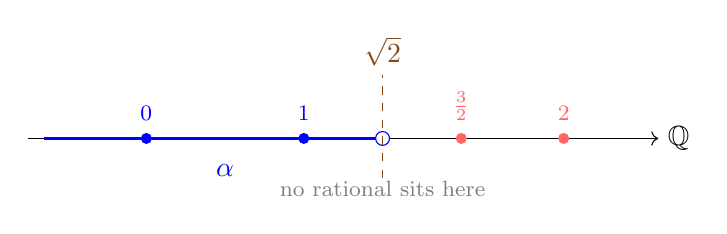
\begin{tikzpicture}[scale=1.0]
    \draw[->] (-1,0) -- (7,0) node[right]{$\mathbb{Q}$};

    % The cut
    \draw[very thick, blue] (-0.8,0) -- (3.5,0);
    \draw[blue, fill=white] (3.5,0) circle (2.5pt);
    \node[blue, below=6pt] at (1.5,0) {$\alpha$};

    % sqrt(2) marker
    \draw[dashed, mAccent] (3.5,-0.5) -- (3.5,0.8);
    \node[mAccent, above] at (3.5,0.8) {$\sqrt{2}$};

    % Some points
    \fill[blue] (0.5,0) circle (2pt) node[above=3pt]{\footnotesize$0$};
    \fill[blue] (2.5,0) circle (2pt) node[above=3pt]{\footnotesize$1$};
    \fill[red!60] (4.5,0) circle (2pt) node[above=3pt]{\footnotesize$\frac{3}{2}$};
    \fill[red!60] (5.8,0) circle (2pt) node[above=3pt]{\footnotesize$2$};

    \node[gray, below=12pt] at (3.5,0) {\footnotesize no rational sits here};
  \end{tikzpicture}
  \end{center}

  \note{
    This example is the whole point of the construction. Remember
    Example 1.1 at the start of the chapter: we proved there is no rational
    whose square equals 2, and this created a "gap" in the rationals. The
    cut on the slide plugs that gap directly. Notice something curious: we
    never mentioned the square root of 2. We defined the cut using only
    rational arithmetic and the inequality "p squared less than 2". The
    irrational number emerges for free as the shape of the cut
    itself. This is the magic of Dedekind's idea --- we get irrationals
    without ever having to refer to them.
  }
\end{frame}

% =============================================================================
% STEP 2: ORDER ON \mathbb{R}
% =============================================================================

\section{Step 2: Ordering the Cuts}

\begin{frame}{Step 2: The Order Relation}
  \begin{defblock}{Definition: Order on $\mathbb{R}$}
    For cuts $\alpha, \beta$, define
    \[
      \alpha < \beta \quad\Longleftrightarrow\quad
      \alpha \subsetneq \beta
      \quad\text{($\alpha$ is a proper subset of $\beta$).}
    \]
  \end{defblock}

  \begin{center}
  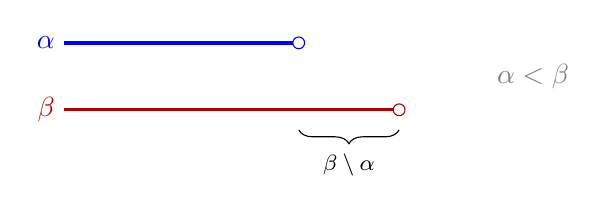
\begin{tikzpicture}[scale=0.85]
    % alpha
    \draw[very thick, blue] (-0.5,0.5) -- (3,0.5);
    \draw[blue, fill=white] (3,0.5) circle (2.5pt);
    \node[blue, left] at (-0.5,0.5) {$\alpha$};

    % beta
    \draw[very thick, red!70!black] (-0.5,-0.5) -- (4.5,-0.5);
    \draw[red!70!black, fill=white] (4.5,-0.5) circle (2.5pt);
    \node[red!70!black, left] at (-0.5,-0.5) {$\beta$};

    % brace for extra part
    \draw[decorate, decoration={brace, amplitude=5pt, mirror}]
      (3,-0.8) -- (4.5,-0.8)
      node[midway, below=5pt]{\footnotesize$\beta \setminus \alpha$};

    % label
    \node[gray] at (6.5,0) {$\alpha < \beta$};
  \end{tikzpicture}
  \end{center}

  \note{
    Here is the elegant economy of the construction: we do not have to
    define an order on the reals because set inclusion already gives
    us one for free. A "smaller" real number reaches less far to the right
    on the number line, so its cut contains fewer rationals. Order is not
    an extra structure we add; it is already encoded in the subset
    relation. This is a recurring theme in mathematics --- the best
    definitions make the hard work disappear. But we still owe a proof
    that inclusion actually satisfies the ordered-set axioms.
  }
\end{frame}

% --- Proof that \mathbb{R} is ordered: Build 1/3 ---
\begin{frame}{Proof: $\mathbb{R}$ Is an Ordered Set}
  \begin{proofblock}{Verification of Definition 1.5}
    \textbf{Transitivity:} If $\alpha < \beta$ and $\beta < \gamma$, then
    $\alpha \subsetneq \beta \subsetneq \gamma$, so $\alpha \subsetneq \gamma$.
      \end{proofblock}

  \note{
    Transitivity is free because subset inclusion is already transitive
    for any sets whatsoever --- it has nothing to do with cuts. We get this
    axiom without paying anything, which is the kind of bonus you hope for
    when your structure is built from well-chosen pieces.
  }
\end{frame}

% --- Proof that \mathbb{R} is ordered: Build 2/3 ---
\begin{frame}{Proof: $\mathbb{R}$ Is an Ordered Set}
  \begin{proofblock}{Verification of Definition 1.5}
    \textbf{Transitivity:} If $\alpha < \beta$ and $\beta < \gamma$, then
    $\alpha \subsetneq \beta \subsetneq \gamma$, so $\alpha \subsetneq \gamma$.
    
    \vspace{0.5em}
    \textbf{At most one holds:} For any $\alpha, \beta$, at most one of
    \[
      \alpha < \beta, \qquad \alpha = \beta, \qquad \beta < \alpha
    \]
    can hold.   \end{proofblock}

  \note{
    This clause is also a freebie from set theory. The real work is
    trichotomy: proving that at least one relation must hold. For general
    sets this would be false --- most pairs of sets are simply
    incomparable. What forces comparability here is the very specific
    shape of a cut, and the next slide is where we finally have to use
    that shape.
  }
\end{frame}

% --- Proof that \mathbb{R} is ordered: Build 3/3 ---
\begin{frame}{Proof: $\mathbb{R}$ Is an Ordered Set}
  \begin{proofblock}{Verification of Definition 1.5}
    \textbf{Transitivity:} If $\alpha < \beta$ and $\beta < \gamma$, then
    $\alpha \subsetneq \beta \subsetneq \gamma$, so $\alpha \subsetneq \gamma$.
    
    \vspace{0.5em}
    \textbf{At most one holds:} For any $\alpha, \beta$, at most one of
    \[
      \alpha < \beta, \qquad \alpha = \beta, \qquad \beta < \alpha
    \]
    can hold.

    \vspace{0.5em}
    \textbf{Trichotomy:} At least one holds.
  \end{proofblock}

  \note{
    Trichotomy is where we have to do actual work. The claim is that any
    two cuts are always comparable. Pause to appreciate how surprising
    this is: arbitrary subsets of the rationals are almost never
    comparable by inclusion, but our cuts always are. Something special
    about the axioms is doing the job.
  }
\end{frame}

% --- Trichotomy diagram ---
\begin{frame}{Proof of Trichotomy --- Key Idea}
  Assume $\alpha \not\subset \beta$. Then some $p \in \alpha$ satisfies
  $p \notin \beta$:

  \begin{center}
  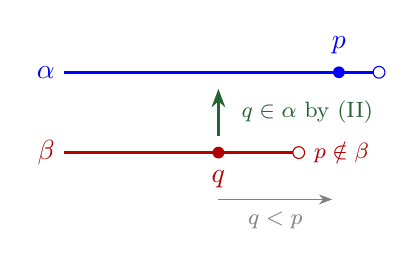
\begin{tikzpicture}[scale=0.85]
    % beta
    \draw[very thick, red!70!black] (-0.5,-0.6) -- (3,-0.6);
    \draw[red!70!black, fill=white] (3,-0.6) circle (2.5pt);
    \node[red!70!black, left] at (-0.5,-0.6) {$\beta$};

    % alpha — extends beyond beta
    \draw[very thick, blue] (-0.5,0.6) -- (4.2,0.6);
    \draw[blue, fill=white] (4.2,0.6) circle (2.5pt);
    \node[blue, left] at (-0.5,0.6) {$\alpha$};

    % p in alpha but not in beta
    \fill[blue] (3.6,0.6) circle (2.5pt);
    \node[blue, above=3pt] at (3.6,0.6) {$p$};

    \node[red!70!black, right=2pt] at (3,-0.6) {\footnotesize$p \notin \beta$};

    % q in beta
    \fill[red!70!black] (1.8,-0.6) circle (2.5pt);
    \node[red!70!black, below=3pt] at (1.8,-0.6) {$q$};

    % arrow: q < p
    \draw[-{Stealth}, gray] (1.8,-1.3) -- (3.5,-1.3);
    \node[gray, below=1pt] at (2.65,-1.3) {\footnotesize$q < p$};

    % arrow: q in alpha
    \draw[-{Stealth}, proofcolor, thick] (1.8,-0.35) -- (1.8,0.35);
    \node[proofcolor, right] at (2.0,0.0) {\footnotesize$q \in \alpha$ by (II)};
  \end{tikzpicture}
  \end{center}

  Since $p \notin \beta$, \emph{every} $q \in \beta$ satisfies $q < p$,
  so $q \in \alpha$.

  \vspace{0.3em}
  Thus $\beta \subset \alpha$, and since $\beta \neq \alpha$:
  $\;\beta < \alpha$.

  \note{
    The strategy is a dichotomy: either "alpha" is contained in "beta" or
    it is not. If it is, we are done. If it is not, we show that "beta"
    must then be contained in "alpha" --- there is no middle ground where
    the two cuts overlap partially. Why? Because a single witness "p" in
    "alpha" but not in "beta" acts like a wall: every element of "beta"
    is forced to sit to the left of "p", and downward closure then sucks
    every such element into "alpha". One escaping point drags the whole
    cut along with it. This leveraging of a single witness is a very
    common proof move; it is worth remembering.
  }
\end{frame}

% --- Trichotomy proof ---
\begin{frame}{Proof of Trichotomy}
  \begin{proofblock}{At least one relation holds}
    Assume $\alpha < \beta$ and $\alpha = \beta$ both fail.

    \vspace{0.3em}
    Then $\alpha \not\subset \beta$, so $\exists\, p \in \alpha$ with
    $p \notin \beta$.

    \vspace{0.3em}
    Pick any $q \in \beta$. Since $p \notin \beta$, we get $q < p$ (by the
    consequence of~(II)).

    \vspace{0.3em}
    Since $q < p$ and $p \in \alpha$, property (II) gives $q \in \alpha$.

    \vspace{0.3em}
    Thus every element of $\beta$ belongs to $\alpha$: $\beta \subset \alpha$.

    \vspace{0.3em}
    Since $\beta \neq \alpha$, we conclude $\beta < \alpha$.   \end{proofblock}

  \note{
    The formal version just spells out the previous picture. Pay
    attention to the logical structure, not the symbols: we started by
    ruling out two of the three possible orderings, and the one witness
    "p" forced the third to hold. That is how trichotomy proofs are
    typically organized --- assume two cases fail and show the third is
    inevitable. With this, the set of cuts is an ordered set, and we can
    move on to its most important structural property.
  }
\end{frame}

% =============================================================================
% STEP 3: LEAST UPPER BOUND PROPERTY
% =============================================================================

\section{Step 3: The Least-Upper-Bound Property}

\begin{frame}{Step 3: The Key Result}
  \begin{thmblock}{Theorem (Step 3)}
    The ordered set $\mathbb{R}$ has the \alert{least-upper-bound property}.
  \end{thmblock}

  \vspace{0.5em}
  \textbf{Strategy:} Given $A \subset \mathbb{R}$ nonempty and bounded above by
  $\beta$, define
  \[
    \gamma \;=\; \bigcup_{\alpha \in A} \alpha
  \]
  and show $\gamma = \sup A$.

    \note{
      This is the payoff for all the care we put into defining cuts.
      Here is why the union works, intuitively. Each cut in "A" is
      a shaded region reaching leftward from some invisible boundary
      point on the number line. When you overlay all of them, the
      result is the shaded region reaching to the rightmost
      boundary among them. That rightmost boundary is exactly the
      supremum. The great surprise is that you never have to
      construct the supremum, you just take a union, and set
      theory does the rest. Compare this with the rationals, where
      no such operation would give you a rational answer --- the
      cut formalism is specifically engineered so that unions stay
      inside the system.
    }
\end{frame}

% --- Proof gamma is a cut: Build 1/3 ---
\begin{frame}{Proof: $\gamma$ Is a Cut}
  \begin{proofblock}{Verifying property (I): $\gamma \neq \emptyset$ and
    $\gamma \neq \mathbb{Q}$}
    \begin{itemize}
      \item $A$ is nonempty, so $\exists\, \alpha_0 \in A$.
            Since $\alpha_0 \neq \emptyset$ and
            $\alpha_0 \subset \gamma$, we get $\gamma \neq \emptyset$.
      \item $\gamma \subset \beta$ (since every $\alpha \in A$ satisfies
            $\alpha \subset \beta$), and $\beta \neq \mathbb{Q}$,
            so $\gamma \neq \mathbb{Q}$.
    \end{itemize}
  \end{proofblock}

  \note{
    Notice how essential the boundedness assumption is here. Without
    the upper bound "beta", the union could in principle swallow all
    of the rationals and fail to be a cut. The upper bound acts like
    a ceiling that confines the union, guaranteeing it stays a
    proper subset. This is why the theorem requires "bounded above"
    --- not just for the conclusion, but for the construction to
    even make sense.
  }
\end{frame}

% --- Proof gamma is a cut: Build 2/3 ---
\begin{frame}{Proof: $\gamma$ Is a Cut}
  \begin{proofblock}{Verifying property (II): if $p \in \gamma$ and $q < p$,
    then $q \in \gamma$}
    Pick $p \in \gamma$. Then $p \in \alpha_1$ for some $\alpha_1 \in A$.

    \vspace{0.3em}
    If $q < p$, then $q \in \alpha_1$ (since $\alpha_1$ is a cut),
    hence $q \in \gamma$.
  \end{proofblock}

  \note{
    Downward closure is inherited automatically: each piece of the
    union is already downward closed, so their union is too. This is
    a general principle worth noting --- unions of downward-closed sets
    stay downward closed, and unions of upward-closed sets stay
    upward closed. Intersections, by contrast, also preserve these
    properties, but unions and intersections behave very differently
    with respect to proper-subset comparisons.
  }
\end{frame}

% --- Proof gamma is a cut: Build 3/3 ---
\begin{frame}{Proof: $\gamma$ Is a Cut}
  \begin{proofblock}{Verifying property (III): $\gamma$ has no largest element}
    Pick $p \in \gamma$. Then $p \in \alpha_1$ for some $\alpha_1 \in A$.

    \vspace{0.3em}
    Since $\alpha_1$ has no largest element, $\exists\, r \in \alpha_1$
    with $r > p$.

    \vspace{0.3em}
    Then $r \in \gamma$ and $r > p$, so $\gamma$ has no largest element.
  \end{proofblock}

  \vspace{0.3em}
  $\boxed{\gamma \in R}$

  \note{
    The no-maximum property also transfers up from the pieces to the
    union for free, and the same general principle applies: a union
    of sets, each without a maximum, cannot have a maximum itself.
    So all three cut axioms are inherited almost automatically from
    the members of "A". The real creativity went into designing the
    axioms; once the axioms are right, verification is mostly
    bookkeeping.
  }
\end{frame}

% --- Proof gamma = sup A ---
\begin{frame}{Proof: $\gamma = \sup A$}
  \begin{proofblock}{$\gamma$ is the least upper bound}
    \textbf{Upper bound:} For every $\alpha \in A$,\;
    $\alpha \subset \gamma$ (by definition of union),
    so $\alpha \leq \gamma$. 
    \vspace{0.5em}
    \textbf{Least:} Suppose $\delta < \gamma$. Then $\exists\, s \in \gamma$
    with $s \notin \delta$.

    \vspace{0.3em}
    Since $s \in \gamma$, we have $s \in \alpha$ for some $\alpha \in A$.

    \vspace{0.3em}
    Hence $\delta < \alpha$, so $\delta$ is \emph{not} an upper bound of $A$.
      \end{proofblock}

  \vspace{0.3em}
  $\boxed{\gamma = \sup A}$

  \note{
    The upper-bound part is trivial by definition of union. The
    "least" part is where the cut formalism really pays off. The
    logic to focus on is this: to show "gamma" is the smallest upper
    bound, we assume someone offers a smaller candidate "delta" and
    we expose it as inadequate by finding an element of "A" that
    escapes above it. That escaping element comes from a single
    rational "s" witnessing "gamma not equal to delta". Once again
    a single point does all the work --- a recurring pattern you
    should start noticing.
  }
\end{frame}

% --- Visual summary ---
\begin{frame}{Visual Summary: $\gamma = \sup A$}
  \begin{center}
  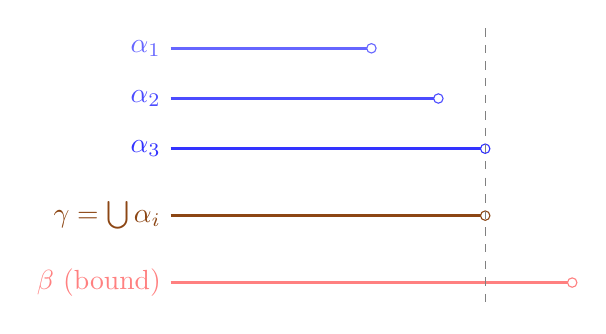
\begin{tikzpicture}[scale=0.85]
    % alpha_1
    \draw[very thick, blue!60] (-0.5,1.5) -- (2.5,1.5);
    \draw[blue!60, fill=white] (2.5,1.5) circle (2pt);
    \node[left, blue!60] at (-0.5,1.5) {$\alpha_1$};

    % alpha_2
    \draw[very thick, blue!70] (-0.5,0.75) -- (3.5,0.75);
    \draw[blue!70, fill=white] (3.5,0.75) circle (2pt);
    \node[left, blue!70] at (-0.5,0.75) {$\alpha_2$};

    % alpha_3
    \draw[very thick, blue!80] (-0.5,0) -- (4.2,0);
    \draw[blue!80, fill=white] (4.2,0) circle (2pt);
    \node[left, blue!80] at (-0.5,0) {$\alpha_3$};

    % gamma = union
    \draw[very thick, mAccent] (-0.5,-1) -- (4.2,-1);
    \draw[mAccent, fill=white] (4.2,-1) circle (2pt);
    \node[left, mAccent] at (-0.5,-1) {$\gamma = \bigcup \alpha_i$};

    % beta (upper bound)
    \draw[very thick, red!50] (-0.5,-2) -- (5.5,-2);
    \draw[red!50, fill=white] (5.5,-2) circle (2pt);
    \node[left, red!50] at (-0.5,-2) {$\beta$ (bound)};

    % Braces
    \draw[dashed, gray] (4.2,1.8) -- (4.2,-2.3);
  \end{tikzpicture}
  \end{center}

  The union $\gamma$ reaches exactly as far as the ``largest'' cut in $A$.

  \note{
    Pause on one subtlety the diagram hides. When "A" is an infinite
    set of cuts, none of them may individually reach all the way up
    to the supremum --- the members may only approach it from
    below, the way one over "n" approaches zero without ever
    touching it. The union still captures the sup exactly, because
    a rational "p" lands in the union if it is in at least one
    member, no matter how late that member appears in the
    enumeration. This is why the construction works even for
    supremums that are not achieved by any single member of "A".
  }
\end{frame}

% =============================================================================
% STEP 4: ADDITION
% =============================================================================

\section{Step 4: Addition of Cuts}

\begin{frame}{Step 4: Defining Addition}
  \begin{defblock}{Definition: Addition of Cuts}
    For cuts $\alpha, \beta \in \mathbb{R}$, define
    \[
      \alpha + \beta \;=\; \{r + s : r \in \alpha,\; s \in \beta\}
    \]
  \end{defblock}

  \vspace{0.5em}
  \begin{defblock}{Definition: The Zero Cut}
    Define $0^* = \{p \in \mathbb{Q} : p < 0\}$.
  \end{defblock}

  \note{
    This definition is the obvious one, but it is worth asking why. If
    cuts represent real numbers, and addition of real numbers should
    correspond to pointwise shifting of boundaries, then the sum of
    cuts should be obtained by sliding the left-hand piece rightward by
    as much as the right-hand piece reaches. Taking all pairwise sums
    achieves exactly that shift without ever mentioning the boundary
    points directly --- which is good, because the boundary points may
    not even exist as rationals. As for "zero star", it is the set of
    rationals strictly less than zero, with zero itself excluded,
    because of the no-maximum axiom.
  }
\end{frame}

% --- Visual: addition of cuts ---
\begin{frame}{Visualizing Cut Addition}
  \begin{center}
  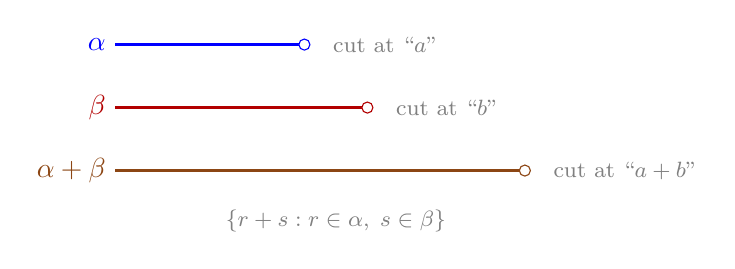
\begin{tikzpicture}[scale=0.8]
    % alpha
    \draw[very thick, blue] (-0.5,2) -- (2.5,2);
    \draw[blue, fill=white] (2.5,2) circle (2.5pt);
    \node[blue, left] at (-0.5,2) {$\alpha$};
    \node[gray, right] at (2.8,2) {\footnotesize cut at ``$a$''};

    % beta
    \draw[very thick, red!70!black] (-0.5,1) -- (3.5,1);
    \draw[red!70!black, fill=white] (3.5,1) circle (2.5pt);
    \node[red!70!black, left] at (-0.5,1) {$\beta$};
    \node[gray, right] at (3.8,1) {\footnotesize cut at ``$b$''};

    % alpha + beta
    \draw[very thick, mAccent] (-0.5,0) -- (6,0);
    \draw[mAccent, fill=white] (6,0) circle (2.5pt);
    \node[mAccent, left] at (-0.5,0) {$\alpha + \beta$};
    \node[gray, right] at (6.3,0) {\footnotesize cut at ``$a + b$''};

    \node[gray] at (3,-0.8) {\footnotesize
      $\{r + s : r \in \alpha,\; s \in \beta\}$};
  \end{tikzpicture}
  \end{center}

  \vspace{0.3em}
  Adding cuts ``adds their boundary points.''

  \note{
    Here is the geometric picture. If "alpha" is the cut at some point "a" and
    "beta" is the cut at some point "b", then "alpha" plus "beta" is the cut at
    "a" plus "b". We take all possible sums of a rational from "alpha" and a
    rational from "beta", and these sums fill out everything to the left of "a"
    plus "b". Of course, we need to verify that this set is actually a cut.
  }
\end{frame}

% --- A1: alpha + beta is a cut: Build 1/3 ---
\begin{frame}{Axiom (A1): $\alpha + \beta$ Is a Cut}
  \begin{proofblock}{Verifying (I): $\alpha + \beta \neq \emptyset$ and
    $\alpha + \beta \neq \mathbb{Q}$}
    $\alpha + \beta$ is nonempty (pick $r \in \alpha$, $s \in \beta$; then
    $r + s \in \alpha + \beta$).

    \vspace{0.3em}
    Take $r' \notin \alpha$, $s' \notin \beta$. For any $r \in \alpha$,
    $s \in \beta$:
    \[
      r < r', \quad s < s' \quad\Longrightarrow\quad r + s < r' + s'
    \]
    So $r' + s' \notin \alpha + \beta$, hence
    $\alpha + \beta \neq \mathbb{Q}$.
  \end{proofblock}

  \note{
    The clever move here is the second half: to show the sum cut is
    not all of the rationals, we build an explicit "ceiling"
    witness. We grab a rational above "alpha" and one above "beta",
    and their sum acts as a ceiling above "alpha plus beta". Why
    does that work? Because sums of smaller things stay smaller
    than sums of larger things --- a trivial fact about the
    rationals, but it is exactly what lets the cut property
    propagate from the inputs to the output. If addition did not
    respect ordering, this whole construction would collapse.
  }
\end{frame}

% --- A1: alpha + beta is a cut: Build 2/3 ---
\begin{frame}{Axiom (A1): $\alpha + \beta$ Is a Cut}
  \begin{proofblock}{Verifying (II): if $p \in \alpha + \beta$ and $q < p$,
    then $q \in \alpha + \beta$}
    Pick $p \in \alpha + \beta$, so $p = r + s$ with $r \in \alpha$,
    $s \in \beta$.

    \vspace{0.3em}
    If $q < p$, then $q - s < r$, so $q - s \in \alpha$ (by~(II) for
    $\alpha$).

    \vspace{0.3em}
    Then $q = (q - s) + s \in \alpha + \beta$.
  \end{proofblock}

  \note{
    The trick is to keep "s" fixed and absorb the shrinkage into
    the "alpha" side. If we want a smaller sum "q", we can write
    "q" as "q minus s" plus "s", treating "s" as a rigid anchor
    and letting the first piece shrink into "alpha" via downward
    closure. This asymmetric move --- freeze one factor, vary the
    other --- appears repeatedly in cut arguments. It works
    because both "alpha" and "beta" are downward closed, so we
    only need to exercise that property on one side.
  }
\end{frame}

% --- A1: alpha + beta is a cut: Build 3/3 ---
\begin{frame}{Axiom (A1): $\alpha + \beta$ Is a Cut}
  \begin{proofblock}{Verifying (III): $\alpha + \beta$ has no largest element}
    Pick $p = r + s \in \alpha + \beta$.

    \vspace{0.3em}
    Choose $t \in \alpha$ with $t > r$ (since $\alpha$ has no largest
    element).

    \vspace{0.3em}
    Then $t + s > r + s = p$ and $t + s \in \alpha + \beta$.   \end{proofblock}

  \vspace{0.3em}
  $\boxed{\alpha + \beta \text{ is a cut}}$

  \note{
    Notice how property 3 of the sum piggybacks on property 3 of
    just one of the summands --- we never even touched "beta".
    Whenever you need to push up slightly above a given element,
    pushing up the "alpha" side is enough. This asymmetry is fine,
    and it shows that the cut axioms are more than we strictly
    need at each step; there is redundancy built in, which makes
    proofs easier.
  }
\end{frame}

% --- A2 through A4 ---
\begin{frame}{Axioms (A2)--(A4): Commutativity, Associativity, Identity}
  \begin{proofblock}{Quick verifications}
    \textbf{(A2) Commutativity:} $\alpha + \beta = \beta + \alpha$

    \hspace{2em}Follows from $r + s = s + r$ in $\mathbb{Q}$.

    \vspace{0.5em}
    \textbf{(A3) Associativity:} $(\alpha + \beta) + \gamma
    = \alpha + (\beta + \gamma)$

    \hspace{2em}Follows from associativity in $\mathbb{Q}$.

    \vspace{0.5em}
    \textbf{(A4) Additive identity:} $\alpha + 0^* = \alpha$

    \hspace{2em}$\subset$: If $r \in \alpha$, $s < 0$, then $r + s < r$,
    so $r + s \in \alpha$.

    \hspace{2em}$\supset$: Pick $p \in \alpha$, choose $r \in \alpha$
    with $r > p$. Then $p - r \in 0^*$ and $p = r + (p-r)$.
  \end{proofblock}

  \note{
    Commutativity and associativity come along for the ride ---
    they inherit from the rationals without any thought, because
    cut addition is defined as pairwise rational addition. The
    interesting axiom is A4. Why is the identity slightly tricky?
    Because "alpha plus zero star" is not literally "alpha"; it
    is a set of sums "r plus s" with "s" negative. It takes a
    little argument to show this set is exactly "alpha", and the
    clever step is the reverse inclusion: given any "p" in
    "alpha", we decompose "p" as "r plus negative number" where
    the larger "r" exists because "alpha" has no maximum. This
    is the first place we use axiom 3 in a nontrivial way.
  }
\end{frame}

% --- A5: Additive inverse - definition ---
\begin{frame}{Axiom (A5): Additive Inverse --- Definition}
  \begin{defblock}{Definition of $-\alpha$}
    For $\alpha \in \mathbb{R}$, define $\beta$ to be the set of all
    $p \in \mathbb{Q}$ such that:

    \vspace{0.3em}
    \emph{There exists $r > 0$ with $-p - r \notin \alpha$.}

    \vspace{0.3em}
    Equivalently: some rational number \emph{strictly less than} $-p$ is not
    in $\alpha$.
  \end{defblock}

  \vspace{0.3em}
  \textbf{High-level idea:} Obtain $-\alpha$ by \alert{flipping the
  "complement"} of $\alpha$ (rationals $> $ boundary) across $0$ (to get
  rationals $< $ -boundary). The buffer $r > 0$ ensures the boundary point
  itself is \emph{excluded} from $-\alpha$.

  \vspace{0.3em}
  \textbf{Goal:} Show $\beta \in \mathbb{R}$ and $\alpha + \beta = 0^*$.

  \note{
    The trickiest axiom is the existence of additive inverses. Given a cut
    "alpha", we need to find a cut "beta" such that "alpha" plus "beta" equals
    "zero star". Here is the high-level idea. The complement of "alpha" consists
    of all rationals that lie at or above its boundary point. If we flip that
    complement across zero, we get exactly the rationals that lie at or below
    the negative of the boundary. That flipped set is almost "minus alpha" ---
    but we do not want the boundary point itself to sneak in. This is why the
    definition introduces a positive buffer "r". By requiring "minus p" minus
    "r" to be outside "alpha", we force "minus p" to sit strictly beyond the
    boundary, not on it. So "p" is in "beta" exactly when some rational strictly
    less than "minus p" fails to be in "alpha". This "beta" is the additive
    inverse of "alpha", denoted "minus alpha".
  }
\end{frame}

% --- A5: Visualising the additive inverse ---
\begin{frame}{Axiom (A5): Visualizing $-\alpha$}
  \begin{center}
  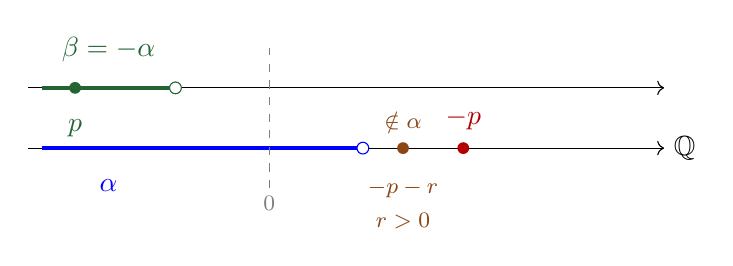
\begin{tikzpicture}[scale=0.85]
    % Number line
    \draw[->] (-1,0) -- (8.5,0) node[right]{$\mathbb{Q}$};

    % alpha
    \draw[very thick, blue] (-0.8,0) -- (4,0);
    \draw[blue, fill=white] (4,0) circle (2.5pt);
    \node[blue, below=8pt] at (0.2,0) {$\alpha$};

    % -p on the number line: to the right of alpha's boundary
    \fill[red!70!black] (5.5,0) circle (2.5pt);
    \node[red!70!black, above=3pt] at (5.5,0) {$-p$};

    % -p - r: strictly less than -p, outside alpha
    \fill[mAccent] (4.6,0) circle (2.5pt);
    \node[mAccent, below=8pt] at (4.6,0) {\footnotesize$-p-r$};
    \node[mAccent, above=3pt] at (4.6,0) {\footnotesize$\notin \alpha$};

    % r > 0 label
    \node[mAccent, below=20pt] at (4.6,0) {\footnotesize$r > 0$};

    % beta = -alpha (on a line slightly above)
    \draw[->] (-1,0.9) -- (8.5,0.9);
    \draw[very thick, proofcolor] (-0.8,0.9) -- (1.2,0.9);
    \draw[proofcolor, fill=white] (1.2,0.9) circle (2.5pt);
    \node[proofcolor, above=6pt] at (0.2,0.9) {$\beta = -\alpha$};

    % p on the beta line
    \fill[proofcolor] (-0.3,0.9) circle (2.5pt);
    \node[proofcolor, below=8pt] at (-0.3,0.9) {$p$};

    % Dashed mirror line at 0
    \draw[dashed, gray] (2.6,-0.6) -- (2.6,1.5);
    \node[gray, below=14pt] at (2.6,0) {\footnotesize$0$};
  \end{tikzpicture}
  \end{center}

  \vspace{0.3em}
  $p \in \beta$ because $-p - r \notin \alpha$: the point $-p$ lies
  \alert{safely beyond} $\alpha$, so $p$ lies safely to the \alert{left of}
  $-\alpha$.

  \note{
    This diagram makes the definition of the additive inverse concrete. On the
    lower number line you see the cut "alpha" in blue, ending at some boundary
    point. On the upper number line you see "beta" equals "minus alpha" in
    green, and the dashed vertical line at zero shows the mirror symmetry
    between the two cuts. Now focus on the point "minus p" on the lower line:
    it sits strictly to the right of "alpha", and "minus p" minus "r" also
    sits outside "alpha", confirming that "minus p" is safely beyond the
    boundary by a buffer of size "r". Reflecting across zero, the point "p"
    lands on the upper line strictly inside "beta". That buffer "r" is the key:
    without it, "p" could land exactly at the boundary of "beta", giving "beta"
    a largest element and ruining the cut property. Now let's verify that
    "beta" is indeed a cut.
  }
\end{frame}

% --- A5: beta is a cut ---
\begin{frame}{Axiom (A5): $\beta = -\alpha$ Is a Cut}
  \begin{proofblock}{Verifying $\beta \in \mathbb{R}$}
    \textbf{(I):} If $s \notin \alpha$, set $p = -s - 1$. Then
    $-p - 1 = s \notin \alpha$, so $p \in \beta$.
    Also $q \in \alpha \Rightarrow -q \notin \beta$, so $\beta \neq \mathbb{Q}$.
    
    \vspace{0.5em}
    \textbf{(II):} If $p \in \beta$ with witness $r > 0$, and $q < p$, then
    $-q - r > -p - r \notin \alpha$, so $q \in \beta$.

    \vspace{0.5em}
    \textbf{(III):} Given $p \in \beta$ with witness $r$, set
    $t = p + r/2$. Then $t > p$ and $-t - r/2 = -p - r \notin \alpha$,
    so $t \in \beta$.   \end{proofblock}

  \note{
    We verify "beta" is a cut. For property 1, pick any "s" not in "alpha"
    and set "p" equals "minus s" minus 1. Then "minus p" minus 1 equals "s",
    which is not in "alpha", so "p" is in "beta". Thus "beta" is nonempty.
    Also, if "q" is in "alpha", then "minus q" cannot be in "beta", because
    every rational less than "q" is already in "alpha", contradicting the
    definition of "beta". So "beta" is not all of the rationals. For property
    2, if "p" is in "beta" and "q" is less than "p", then "minus q" is
    greater than "minus p", so the same witness "r" works for "q". For
    property 3, given the witness "r", we take "t" equals "p" plus "r"
    over 2, which is strictly greater than "p" and still in "beta" with
    witness "r" over 2. Now we must show that "alpha" plus "beta" equals
    "zero star".
  }
\end{frame}

% --- A5: alpha + beta = 0* ---
\begin{frame}{Axiom (A5): Proof that $\alpha + \beta = 0^*$}
  \begin{proofblock}{$\alpha + \beta \subset 0^*$}
    If $r \in \alpha$ and $s \in \beta$, then $-s \notin \alpha$, so $r < -s$,
    hence $r + s < 0$.
  \end{proofblock}

  \vspace{0.3em}
  \begin{proofblock}{$0^* \subset \alpha + \beta$}
    \textbf{High-level idea:} Pick $v < 0$. Write $v = v/2 + v/2$ and split it
    as $v = (v/2 + t) + (v/2 - t)$, $t > 0$ chosen so that
    $v/2 + t \in \alpha$ and $v/2 - t \in \beta$.

    \vspace{0.2em}
    Set $w = -v/2 > 0$.
    By the Archimedean property of $\mathbb{Q}$, $\exists\, n$ such that
    $nw \in \alpha$ but $(n+1)w \notin \alpha$.

    \vspace{0.2em}
    Take $t = (n+1)w$. Then $v/2 + t = nw \in \alpha$, and
    $p := v/2 - t = -(n+2)w$ satisfies $-p - w = (n+1)w \notin \alpha$,
    so $p \in \beta$. Hence $v = nw + p \in \alpha + \beta$.
  \end{proofblock}

  \note{
    We show "alpha" plus "beta" equals "zero star" in two parts. The forward
    inclusion is clean: if "r" is in "alpha" and "s" is in "beta", then "minus
    s" is not in "alpha", so "r" is less than "minus s", which gives "r" plus
    "s" less than zero. For the reverse inclusion, here is the high-level idea.
    Given a negative rational "v", we want to write it as a sum of something in
    "alpha" and something in "beta". The trick is to split "v" symmetrically as
    "v" over 2 plus "t", and "v" over 2 minus "t", for some cleverly chosen
    positive "t". We want the first piece to land inside "alpha", and the
    second piece to land inside "beta". To find this "t", we use the
    Archimedean property. Set "w" to be "minus v" over 2, which is positive.
    The Archimedean property gives an integer "n" such that "n" times "w" is
    in "alpha" but "n" plus 1 times "w" is not. This "n" marks the boundary of
    "alpha" on the lattice of multiples of "w". Now take "t" equal to "n" plus
    1 times "w". Then "v" over 2 plus "t" simplifies to "n" times "w", which
    is in "alpha". And "v" over 2 minus "t" equals minus "n" plus 2 times "w",
    call it "p". To check "p" is in "beta", note that "minus p" minus "w"
    equals "n" plus 1 times "w", which is outside "alpha" --- exactly the
    witness "beta" requires. So "v" equals "n" times "w" plus "p" belongs to
    "alpha" plus "beta". This completes the proof that "beta" is the additive
    inverse, which we denote "minus alpha".
  }
\end{frame}

% --- A5: Visualising the splitting idea ---
\begin{frame}{Axiom (A5): Visualizing $0^* \subset \alpha + \beta$}
  \begin{center}
  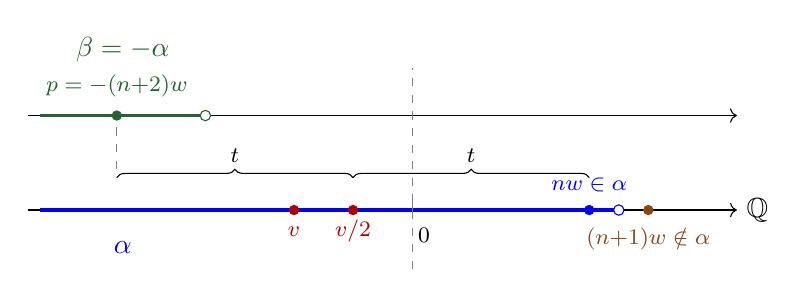
\begin{tikzpicture}[scale=0.75]
    % Alpha number line
    \draw[->] (-6.5,0) -- (5.5,0) node[right]{$\mathbb{Q}$};

    % alpha cut (up to boundary 3.5)
    \draw[very thick, blue] (-6.3,0) -- (3.5,0);
    \draw[blue, fill=white] (3.5,0) circle (2.5pt);
    \node[blue, below=8pt] at (-4.9,0) {$\alpha$};

    % zero tick
    \draw[thin, gray] (0,-0.15) -- (0,0.15);
    \node[black, below=3pt] at (0.2,0) {\footnotesize$0$};

    % lattice: nw in alpha, (n+1)w outside
    \fill[blue] (3,0) circle (2.5pt);
    \node[blue, above=3pt] at (3,0) {\footnotesize$nw \in \alpha$};

    \fill[mAccent] (4,0) circle (2.5pt);
    \node[mAccent, below=3pt] at (4,0) {\footnotesize$(n{+}1)w \notin \alpha$};

    % v on alpha line
    \fill[red!70!black] (-2,0) circle (2.5pt);
    \node[red!70!black, anchor=base] at (-2,-0.45) {\footnotesize$v$};

    % v/2 on alpha line (midpoint of p and nw)
    \fill[red!70!black] (-1,0) circle (2.5pt);
    \node[red!70!black, anchor=base] at (-1,-0.45) {\footnotesize$v/2$};

    % Equidistance braces above alpha line
    \draw[decorate, decoration={brace, amplitude=3pt}]
      (-5,0.55) -- (-1,0.55) node[midway, above=2pt]{\footnotesize$t$};
    \draw[decorate, decoration={brace, amplitude=3pt}]
      (-1,0.55) -- (3,0.55) node[midway, above=2pt]{\footnotesize$t$};

    % beta line above (boundary at -3.5, exact mirror of alpha's 3.5)
    \draw[->] (-6.5,1.6) -- (5.5,1.6);
    \draw[very thick, proofcolor] (-6.3,1.6) -- (-3.5,1.6);
    \draw[proofcolor, fill=white] (-3.5,1.6) circle (2.5pt);
    \node[proofcolor, above=16pt] at (-4.9,1.6) {$\beta = -\alpha$};

    % mirror dashed line at 0
    \draw[dashed, gray] (0,-1.0) -- (0,2.4);

    % dashed drop from p down to brace level (showing horizontal alignment)
    \draw[dashed, gray] (-5,1.4) -- (-5,0.55);

    % p on beta line
    \fill[proofcolor] (-5,1.6) circle (2.5pt);
    \node[proofcolor, above=3pt] at (-5,1.6) {\footnotesize$p = -(n{+}2)w$};
  \end{tikzpicture}
  \end{center}

  \vspace{0.2em}
  $v/2$ sits \alert{exactly halfway} between $p$ and $nw$: shifting by
  $t = (n+1)w$ to the right lands at $nw \in \alpha$, shifting by $t$ to
  the left lands at $p \in \beta$.

  \note{
    This diagram visualizes the clever splitting. On the bottom number line we
    see the cut "alpha" in blue, extending to the left up to its boundary. On
    top we see "beta" equals "minus alpha" in green, extending to the left up
    to the mirror image of that boundary across zero. The Archimedean property
    gives us an integer "n" such that "n" times "w" lands inside "alpha",
    shown as the blue dot, while "n" plus 1 times "w" lands just outside,
    shown as the brown dot. These two lattice points bracket the boundary of
    "alpha" from both sides. Now pay attention to the midpoint "v" over 2,
    shown on the lower line. The two braces above the line show that "v" over
    2 is equidistant from "nw" on the right and from "p" on the left, at
    distance exactly "t" equals "n" plus 1 times "w". In other words, "v"
    over 2 plus "t" equals "nw", which lives inside "alpha", and "v" over 2
    minus "t" equals "p", which lives inside "beta" on the upper line. Adding
    these two pieces recovers the target "v". So "v" has been exhibited as
    the sum of something in "alpha" and something in "beta", exactly what we
    needed.
  }
\end{frame}

% =============================================================================
% STEP 5: ORDER AND ADDITION
% =============================================================================

\section{Step 5: Order Compatibility with Addition}

\begin{frame}{Step 5: Addition Preserves Order}
  \begin{thmblock}{Proposition (Step 5)}
    If $\alpha, \beta, \gamma \in \mathbb{R}$ and $\beta < \gamma$, then
    $\alpha + \beta < \alpha + \gamma$.
  \end{thmblock}

  \vspace{0.5em}
  \begin{proofblock}{Proof}
    From the definition of $+$:
    $\alpha + \beta \subset \alpha + \gamma$ is clear.

    \vspace{0.3em}
    If $\alpha + \beta = \alpha + \gamma$, the cancellation law
    (Proposition 1.14) gives $\beta = \gamma$. Contradiction.

    \vspace{0.3em}
    Thus $\alpha + \beta \subsetneq \alpha + \gamma$, i.e.,
    $\alpha + \beta < \alpha + \gamma$.   \end{proofblock}

  \note{
    This is the compatibility axiom that turns an ordered ring into
    an ordered field in the sense of Definition 1.17. The
    interesting question is not that the proof is short --- it is
    why it is short. The answer: inclusion between cuts really is
    the order, and union-like operations preserve inclusion
    automatically. Once we know cancellation, getting
    strict inequality instead of just weak inequality is immediate.
    Contrast this with what happens if you try to verify the same
    axiom on the Cauchy-sequence construction of the reals --- it
    is much messier there.
  }
\end{frame}

\begin{frame}{Step 5: Consequence}
  \begin{remblock}{Remark}
    It also follows that
    \[
      \alpha > 0^* \quad\Longleftrightarrow\quad -\alpha < 0^*.
    \]
  \end{remblock}

  \vspace{0.5em}
  With Steps 4 and 5, the first requirement of an ordered field
  (Definition~1.17) is satisfied.

  \note{
    As a consequence, a cut is positive if and only if its additive inverse is
    negative. With the addition axioms verified and order compatibility
    established, we have confirmed the first requirement of Definition 1.17.
    Now we need to handle multiplication, which is the subject of the next two
    steps.
  }
\end{frame}

% =============================================================================
% STEPS 6--7: MULTIPLICATION
% =============================================================================

\section{Steps 6--7: Multiplication}

\begin{frame}{Step 6: Multiplication for Positive Cuts}
  \begin{defblock}{Definition: Multiplication on $\mathbb{R}^+$}
    For $\alpha, \beta \in \mathbb{R}^+$ (i.e., $\alpha > 0^*$ and $\beta > 0^*$),
    define $\alpha\beta$ to be the set of all $p \in \mathbb{Q}$ such that
    \[
      p \leq rs \quad\text{for some } r \in \alpha,\; s \in \beta,\;
      r > 0,\; s > 0.
    \]
  \end{defblock}

  \vspace{0.5em}
  \begin{defblock}{Definition: The Unit Cut}
    $1^* = \{q \in \mathbb{Q} : q < 1\}$
  \end{defblock}

  \note{
    A warning about why multiplication is harder than addition. For
    addition, the pairwise-sum idea works uniformly because sums of
    smaller numbers are always smaller --- addition preserves order
    with no exceptions. But multiplication flips sign: multiplying
    by a negative reverses order. So the naive "pairwise product"
    set would not even be downward closed if negatives were allowed.
    The standard dodge is to define multiplication first on positive
    cuts, where order is preserved, and then handle signs by hand
    in Step 7. Another small detail: notice the definition uses "p
    less than or equal to "r s", not strict, to ensure downward
    closure works cleanly.
  }
\end{frame}

\begin{frame}{Step 6: Axioms (M) and (D) on $\mathbb{R}^+$}
  \begin{proofblock}{Verification}
    The axioms (M) of Definition 1.12 hold in $\mathbb{R}^+$ with $1^*$ as the
    identity:
    \begin{itemize}
      \item[(M1)] $\alpha\beta$ is a cut (closure)
      \item[(M2)] $\alpha\beta = \beta\alpha$ (commutativity)
      \item[(M3)] $(\alpha\beta)\gamma = \alpha(\beta\gamma)$ (associativity)
      \item[(M4)] $\alpha \cdot 1^* = \alpha$ (identity)
      \item[(M5)] Multiplicative inverses exist in $\mathbb{R}^+$
    \end{itemize}

    \vspace{0.3em}
    The distributive law (D) also holds in $\mathbb{R}^+$.
  \end{proofblock}

  \vspace{0.3em}
  The proofs parallel the addition axioms from Step~4.

  \note{
    Rudin skips these proofs because they are mechanical repetitions
    of the addition arguments, but it is worth mentioning what is
    different. Multiplicative inverses are the one genuinely novel
    step: you have to invert the boundary point of "alpha" across
    1 rather than across 0, and the same "buffer" trick from the
    additive inverse reappears. If you sit down to do the work
    yourself, expect the inverse axiom to be harder than all the
    others combined --- the same way it was for addition.
  }
\end{frame}

% --- Step 7: extending multiplication ---
\begin{frame}{Step 7: Extending Multiplication to All of $\mathbb{R}$}
  \begin{defblock}{Definition: Full Multiplication}
    Set $\alpha \cdot 0^* = 0^* \cdot \alpha = 0^*$ for all $\alpha$, and:
    \[
      \alpha\beta = \begin{cases}
        (-\alpha)(-\beta)
          & \text{if } \alpha < 0^*,\; \beta < 0^* \\[4pt]
        -[(-\alpha)\beta]
          & \text{if } \alpha < 0^*,\; \beta > 0^* \\[4pt]
        -[\alpha \cdot (-\beta)]
          & \text{if } \alpha > 0^*,\; \beta < 0^*
      \end{cases}
    \]
  \end{defblock}

  \note{
    This is the rule-of-signs definition, imposed by hand rather than
    derived from a general construction. It feels ad hoc, and in a
    sense it is --- but there is no better option. Any definition of
    multiplication that handles negatives uniformly would require
    the sign-flipping property to be derivable from something else,
    and when you are constructing the reals from scratch there is
    nothing else yet to derive it from. The lesson is that the
    familiar "negative times negative equals positive" rule is not
    a fact about numbers; it is a choice that makes the
    distributive law hold.
  }
\end{frame}

\begin{frame}{Step 7: Completing the Ordered Field}
  \begin{proofblock}{Verification}
    The axioms (M) extend from $\mathbb{R}^+$ to all of $\mathbb{R}$ using the identity
    $\gamma = -(-\gamma)$ (Proposition 1.14).

    \vspace{0.5em}
    The \textbf{distributive law} $\alpha(\beta + \gamma) = \alpha\beta + \alpha\gamma$
    is verified by cases on the signs of $\alpha$, $\beta$, $\beta + \gamma$.
  \end{proofblock}

  \vspace{0.5em}
  \begin{thmblock}{Conclusion of Steps 1--7}
    $\mathbb{R}$ is an \alert{ordered field} with the \alert{least-upper-bound property}.
  \end{thmblock}

  \note{
    Why does case analysis work here at all? Because the
    distributive law in the positive case --- which we already know
    --- propagates outward through all the sign combinations via the
    identity that negation commutes with multiplication. In other
    words, the whole field structure on "R" is bootstrapped
    from the positive-cut calculations in Step 6. This is a nice
    instance of a general technique: prove the theorem in the
    simplest regime, then use symmetry to extend. Steps 1 through 7
    now deliver everything Theorem 1.19 promised about existence.
    All that remains is the embedding of the rationals.
  }
\end{frame}

% =============================================================================
% STEPS 8--9: EMBEDDING Q INTO \mathbb{R}
% =============================================================================

\section{Steps 8--9: Embedding $\mathbb{Q}$ into $\mathbb{R}$}

\begin{frame}{Step 8: Rational Cuts}
  \begin{defblock}{Definition: Rational Cuts}
    For each $r \in \mathbb{Q}$, define
    \[
      r^* = \{p \in \mathbb{Q} : p < r\}.
    \]
  \end{defblock}

  \vspace{0.3em}
  Each $r^*$ is a cut (easy to verify). These are the \alert{rational cuts}.

  \begin{center}
  \begin{tikzpicture}[scale=0.9]
    \draw[->] (-0.5,0) -- (7,0) node[right]{$\mathbb{Q}$};
    \draw[very thick, blue] (-0.3,0) -- (3.5,0);
    \draw[blue, fill=white] (3.5,0) circle (2.5pt);
    \fill[mAccent] (3.5,0.3) circle (0pt) node[above]{\footnotesize$r$};
    \node[blue, below=6pt] at (1.5,0) {$r^*$};
    \node[gray, below=6pt] at (5.2,0) {$\mathbb{Q}\setminus r^*$};
  \end{tikzpicture}
  \end{center}

  \note{
    There is a potential for confusion here. The rational number "r"
    and the rational cut "r star" are not the same thing:
    "r" is a number, "r star" is a set of numbers. But they will
    behave identically under addition, multiplication, and
    comparison, and that is all the algebra can see. This
    distinction matters philosophically but becomes invisible in
    practice, which is exactly why we can afterwards pretend that
    the rationals live inside the reals. Also note why the
    no-maximum axiom forces the strict inequality: if we allowed
    "p equals r" into the cut, it would be the largest element.
  }
\end{frame}

% --- Properties of rational cuts: Build 1/3 ---
\begin{frame}{Step 8: Properties of Rational Cuts}
  \begin{thmblock}{Properties}
    For $r, s \in \mathbb{Q}$:
    \begin{enumerate}
      \item[(a)] $r^* + s^* = (r + s)^*$
    \end{enumerate}
  \end{thmblock}

  \vspace{0.3em}
  \begin{proofblock}{Proof of (a)}
    $(\subset)$\; If $p = u + v$ with $u < r$, $v < s$, then $p < r + s$.\;
    $(\supset)$\; If $p < r + s$, set $t = (r + s - p)/2$, then
    $r' = r - t \in r^*$, $s' = s - t \in s^*$, and $p = r' + s'$.
  \end{proofblock}

  \note{
    This is the step that promotes the map "r goes to r star" from
    a mere bijection to a genuine homomorphism. The forward
    inclusion is trivial; the reverse is the interesting direction,
    and the trick is that when "p" strictly undershoots "r plus s",
    we have positive room to spare --- namely the gap "t". We
    split that gap evenly between the two sides, and both halves
    land safely inside their respective rational cuts. Dividing
    the slack in half is a small move, but it is the heart of the
    proof, and it only works because the rationals are densely
    ordered.
  }
\end{frame}

% --- Properties of rational cuts: Build 2/3 ---
\begin{frame}{Step 8: Properties of Rational Cuts}
  \begin{thmblock}{Properties}
    For $r, s \in \mathbb{Q}$:
    \begin{enumerate}
      \item[(a)] $r^* + s^* = (r + s)^*$
      \item[(b)] $r^* \cdot s^* = (rs)^*$
    \end{enumerate}
  \end{thmblock}

  \vspace{0.3em}
  The proof of (b) is similar to (a).

  \note{
    The second property says that multiplying rational cuts corresponds to
    multiplying the rationals. The proof follows the same pattern as part (a).
    The third and final property concerns order.
  }
\end{frame}

% --- Properties of rational cuts: Build 3/3 ---
\begin{frame}{Step 8: Properties of Rational Cuts}
  \begin{thmblock}{Properties}
    For $r, s \in \mathbb{Q}$:
    \begin{enumerate}
      \item[(a)] $r^* + s^* = (r + s)^*$
      \item[(b)] $r^* \cdot s^* = (rs)^*$
      \item[(c)] $r^* < s^*$ if and only if $r < s$
    \end{enumerate}
  \end{thmblock}

  \vspace{0.3em}
  \begin{proofblock}{Proof of (c)}
    If $r < s$: then $r \in s^*$ but $r \notin r^*$, so $r^* \subsetneq s^*$.

    \vspace{0.2em}
    If $r^* < s^*$: $\exists\, p \in s^*$ with $p \notin r^*$, so
    $r \leq p < s$, giving $r < s$.
  \end{proofblock}

  \note{
    The key witness in the forward direction is "r" itself: it is
    strictly below "s" so it lives in "s star", but it is not
    strictly below itself so it is not in "r star". That
    single rational separates the two cuts, proving proper
    containment. In the reverse direction we again use a single
    witness to translate a set-theoretic statement back into an
    inequality on rationals. With these three properties, we can
    stop distinguishing "r" from "r star" --- the embedding is
    faithful in every way we care about.
  }
\end{frame}

% --- Step 9: identification ---
\begin{frame}{Step 9: $\mathbb{Q}$ as a Subfield of $\mathbb{R}$}
  \begin{remblock}{Key Observation}
    The map $r \mapsto r^*$ from $\mathbb{Q}$ to $\mathbb{R}$ preserves:
    \begin{itemize}
      \item Sums: $r^* + s^* = (r+s)^*$
      \item Products: $r^* \cdot s^* = (rs)^*$
      \item Order: $r < s \iff r^* < s^*$
    \end{itemize}

    \vspace{0.3em}
    We say $\mathbb{Q}$ is \alert{isomorphic} to
    $\mathbb{Q}^* = \{r^* : r \in \mathbb{Q}\}$.
  \end{remblock}

  \vspace{0.3em}
  \emph{This identification allows us to regard $\mathbb{Q}$ as a subfield
  of~$\mathbb{R}$.}

  \note{
    Step 9 puts everything together. The rational cuts form a subset of "R"
    that behaves exactly like the rationals: addition, multiplication, and
    order all match up. While "r" star is technically a set of rationals, not
    the rational number "r" itself, all the algebraic and order properties are
    identical. This is what isomorphic means. From now on, we can safely
    identify each rational "r" with its cut "r" star and think of the rationals
    as sitting inside the reals.
  }
\end{frame}

\begin{frame}{Step 9: Uniqueness and Historical Notes}
  \begin{remblock}{Uniqueness}
    Any two ordered fields with the least-upper-bound property are
    \alert{isomorphic}.

    \vspace{0.3em}
    Thus Theorem 1.19 \emph{characterizes} $\mathbb{R}$ completely.
  \end{remblock}

  \vspace{0.5em}
  \textbf{Historical note:}
  \begin{itemize}
    \item \textbf{Dedekind} (1872): Construction via cuts (the one we just saw)
    \item \textbf{Cantor} (1872): Construction via Cauchy sequences of
          rationals
  \end{itemize}

  \note{
    A remarkable fact, which Rudin states without proof, is that any two
    ordered fields with the least-upper-bound property are isomorphic. This
    means there is essentially only one such field: the real numbers. Our
    construction via Dedekind cuts is one way to build it; Cantor's
    construction using equivalence classes of Cauchy sequences is another.
    Both were published in 1872. The two approaches are quite different in
    flavor, but they produce isomorphic results.
  }
\end{frame}

% =============================================================================
% SUMMARY
% =============================================================================

\section{Summary}

% --- Summary: Build 1/4 ---
\begin{frame}{Summary}
  \textbf{Key takeaways from this appendix:}
  \begin{itemize}
    \item A \alert{Dedekind cut} is a nonempty, proper, downward-closed subset
          of $\mathbb{Q}$ with no largest element
  \end{itemize}

  \note{
    Let's review the key ideas from this appendix. First, a Dedekind cut is a
    subset of the rationals satisfying three simple properties: it is nonempty
    and proper, it is closed downward, and it has no largest element. And the
    key consequence of this definition is next.
  }
\end{frame}

% --- Summary: Build 2/4 ---
\begin{frame}{Summary}
  \textbf{Key takeaways from this appendix:}
  \begin{itemize}
    \item A \alert{Dedekind cut} is a nonempty, proper, downward-closed subset
          of $\mathbb{Q}$ with no largest element
    \item The set $\mathbb{R}$ of all cuts, ordered by inclusion, has the
          \alert{least-upper-bound property} (the supremum is the union)
  \end{itemize}

  \note{
    The set of all cuts, ordered by inclusion, automatically has the
    least-upper-bound property. The supremum of a bounded set of cuts is just
    their union. This is the central insight of the construction. But we also
    needed arithmetic.
  }
\end{frame}

% --- Summary: Build 3/4 ---
\begin{frame}{Summary}
  \textbf{Key takeaways from this appendix:}
  \begin{itemize}
    \item A \alert{Dedekind cut} is a nonempty, proper, downward-closed subset
          of $\mathbb{Q}$ with no largest element
    \item The set $\mathbb{R}$ of all cuts, ordered by inclusion, has the
          \alert{least-upper-bound property} (the supremum is the union)
    \item With addition and multiplication defined on cuts, $\mathbb{R}$ becomes an
          \alert{ordered field}
  \end{itemize}

  \note{
    By defining addition as pairwise sums and multiplication carefully by
    cases, the set of cuts becomes a full ordered field. And the final piece
    of the puzzle is the connection to the rationals.
  }
\end{frame}

% --- Summary: Build 4/4 ---
\begin{frame}{Summary}
  \textbf{Key takeaways from this appendix:}
  \begin{itemize}
    \item A \alert{Dedekind cut} is a nonempty, proper, downward-closed subset
          of $\mathbb{Q}$ with no largest element
    \item The set $\mathbb{R}$ of all cuts, ordered by inclusion, has the
          \alert{least-upper-bound property} (the supremum is the union)
    \item With addition and multiplication defined on cuts, $\mathbb{R}$ becomes an
          \alert{ordered field}
    \item The rational cuts $r^* = \{p \in \mathbb{Q} : p < r\}$ embed
          $\mathbb{Q}$ as a subfield of $\mathbb{R}$, completing the proof of
          Theorem~1.19
  \end{itemize}

  \vspace{0.5em}
  \textbf{Coming up next:} Chapter 2 --- Basic Topology.

  \note{
    Finally, every rational number corresponds to a rational cut, and this
    correspondence preserves all arithmetic and order. This completes the
    construction of the real numbers and the proof of Theorem 1.19. With the
    real number system firmly established, we are ready to move on to Chapter 2,
    where we study the topology of metric spaces, including the crucial
    concepts of open sets, closed sets, and compactness.
  }
\end{frame}

\end{document}
